To access the web application, navigate to a domain and directory that publicly serves the web page. An example of this is the “official” test enviroment: www8.cs.umu.se/~oi11lsm/app/.
All functionality of the web application is (or rather should be) fairly self-explanatory and intuitive. A short description and explanation will be given for each component that have been implemented so far.
\subsection{Using the interface}
This section will describe how to use the interface and how to interact with it.
\subsubsection{Start view}
%figure 2
\begin{figure}[h]
\centering
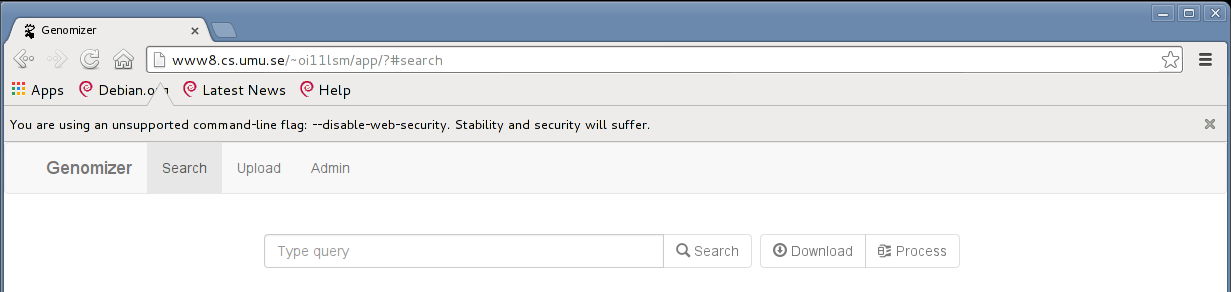
\includegraphics[width=1\textwidth]{web_search_welcome.png}
\caption{\label{fig:web_search_welcome} The welcome screen of the webpage.}
\end{figure}

When the website has loaded, the user is taken to the search page as shown in \refer{fig:web_search_welcome}.

The navigation bar at the top has three buttons with the following functionality:
\begin{itemize}
	\item Clicking the “Genomizer” logo should take the user right back to the start view.
	\item The “Search” button will bring up the search view where the user can enter search strings to be sent to the server, and view search results.
	\item The “Upload” button will bring up the upload view where the user can select files to be uploaded and input annotation to a new experiment.
	\item The “Admin” button will be shown for administrators, that is where the administrator can handle users and annotations.
\end{itemize}
This navigation bar is persistent through all subpages and can easily be accessed.

Below the navigation bar a “search-and-functionality” bar is visible, there is a search field and there are three buttons, Search, Download and process. However, when first entering the page the buttons will be disabled. When you enter something in the search field the search button will become enabled and clickable. 
When the user wants to search for something he can simply write a search query in pubmed style(ex; Exp1[ExpID]) in the search field and either press enter or click the Search button. 

%figure BILD
\begin{figure}[h]
\centering
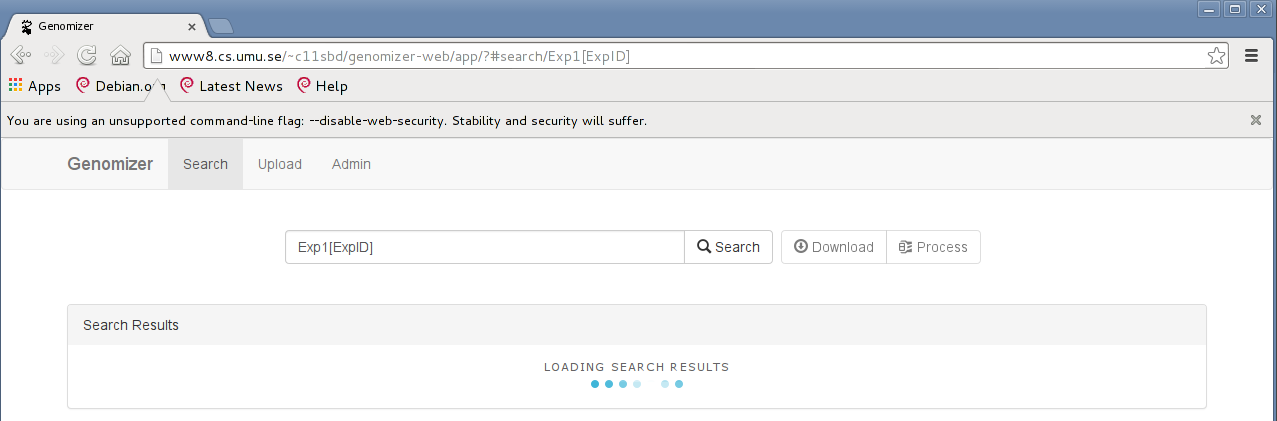
\includegraphics[width=1\textwidth]{web_search_searching.png}
\caption{\label{fig:web_search_searching}will be shown while searching for data in the database before any results are found.}
\end{figure}

After having typed a query and pressed search, the search results will load displaying the loading spinner as can be seen in figure \refer{fig:web_search_searching}.
%figure x3
\begin{figure}[h]
\centering
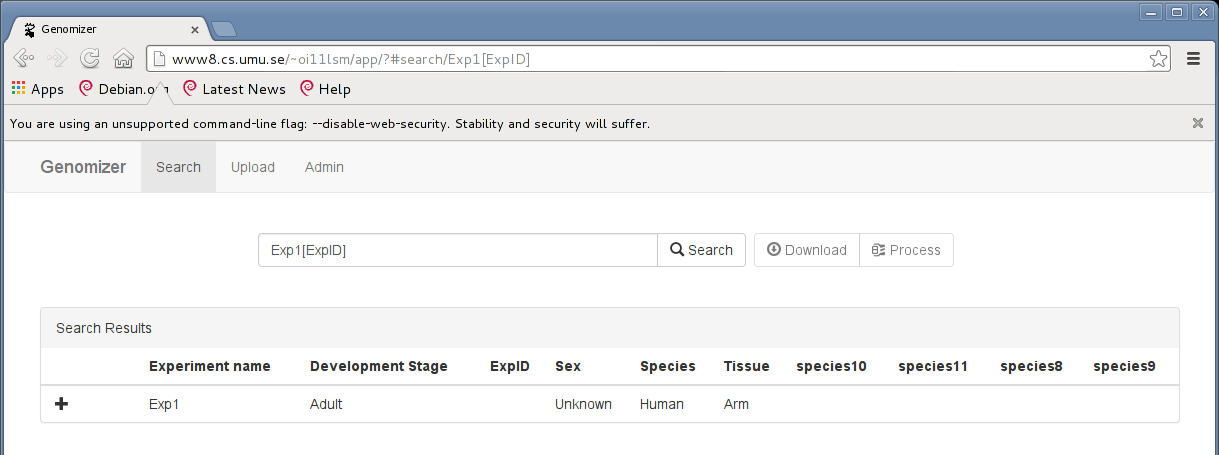
\includegraphics[width=1\textwidth]{web_search_searchTab.png}
\caption{\label{fig:web_search_searchTab}the search tab after a search for ‘Exp1[ExpID]’.}
\end{figure}

The view shown in \refer{fig:web_search_searchTab} contains two major elements; a “search-and-functionality” bar and a list of search results retrieved after searching for ‘Exp1[ExpID]’. The buttons next to the search bar are supposed to do what they say: 
\begin{itemize}
	\item “Search” searches for the query in the search bar. 
	\item “Download” downloads the selected files. 
	\item “Process” brings up a new window in front of the search view with options for file processing. This feature is demonstrated further in Figure \refer{fig:web_process_modal}.
\end{itemize}

Below the search bar in \refer{fig:web_search_searchTab} is the “search results” list. This list contains all experiments returned from a search. Every experiment can be expanded to show the file types it contains,. Each file type can be expanded to show all files of that type in the experiment. Each file has a check box next to it that is used to select files to be processed or downloaded, currently the user is only able to select one file at a time. 
%figure x4
\begin{figure}[h]
\centering
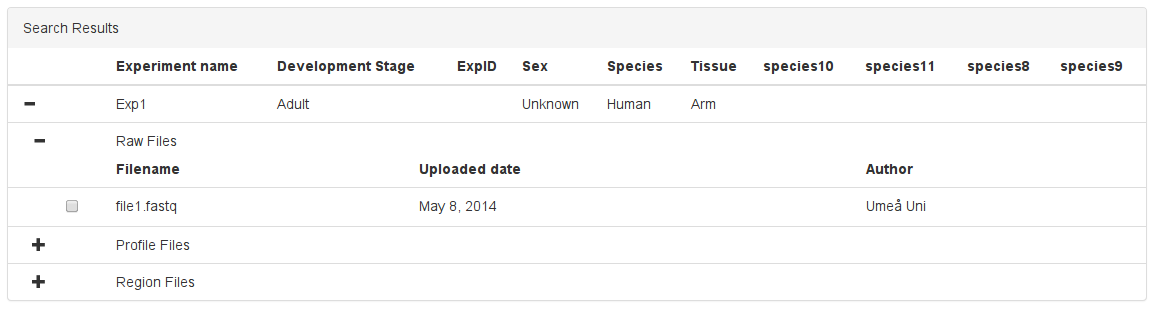
\includegraphics[width=1\textwidth]{web_search_searchResult.png}
\caption{\label{fig:web_search_searchResult}the search results table zoomed in, displaying a raw file’s information after having expanded an experiment.}
\end{figure}

If a search is successful, you will be met with a table of results. This table has a header displaying the annotation types. Below that, all the experiments returned from a search and their corresponding annotation values, as can be seen in \refer{fig:web_search_searchResult}.
%figure BILD PÅ NO SEARCH RESULTS
\begin{figure}[h]
\centering
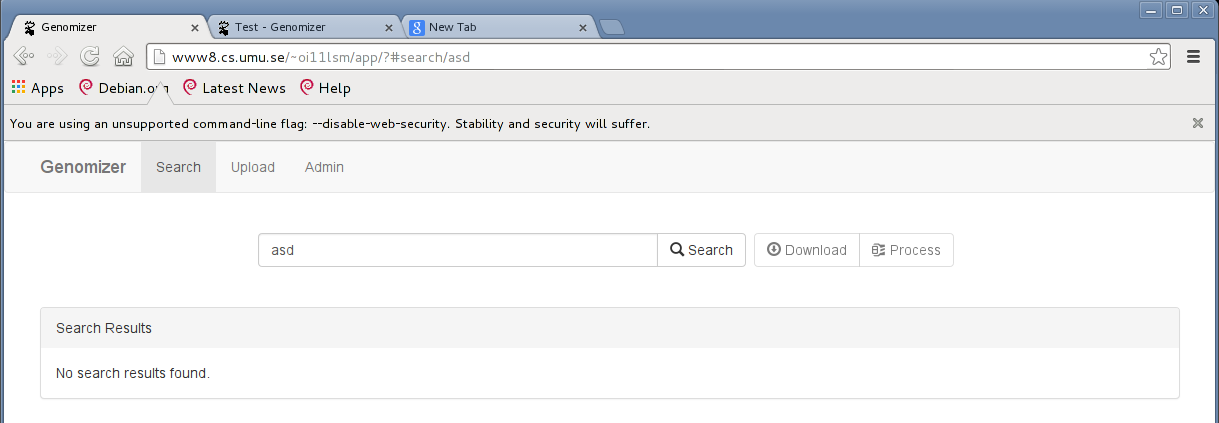
\includegraphics[width=1\textwidth]{web_search_noResult.png}
\caption{\label{fig:web_search_noResult}tells the user that no data was found given the search query entered by the user.}
\end{figure}

If the search is unsuccessful, the Search Results table will be empty stating “No search results found” as can be seen in \refer{fig:web_search_noResult}.

\subsubsection{The processing modal}
%figure X6
\begin{figure}[ht]
\centering
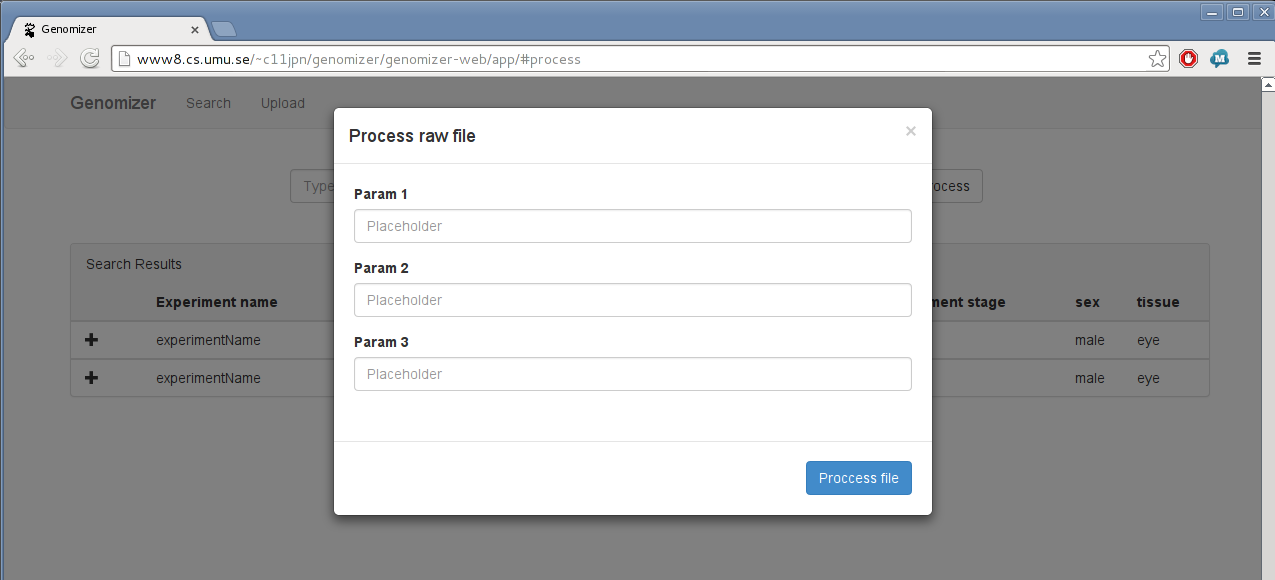
\includegraphics[width=1\textwidth]{web_process_modal.png}
\caption{\label{fig:web_process_modal}The process file modal.}
\end{figure}

The user will be presented with the view in \refer{fig:web_process_modal} when he wants to process one raw file to profile data. The user will already have selected one file he wishes to process and he will enter the parameters for the processing.
\subsubsection{The upload view}
%figure X7
\begin{figure}[h]
\centering
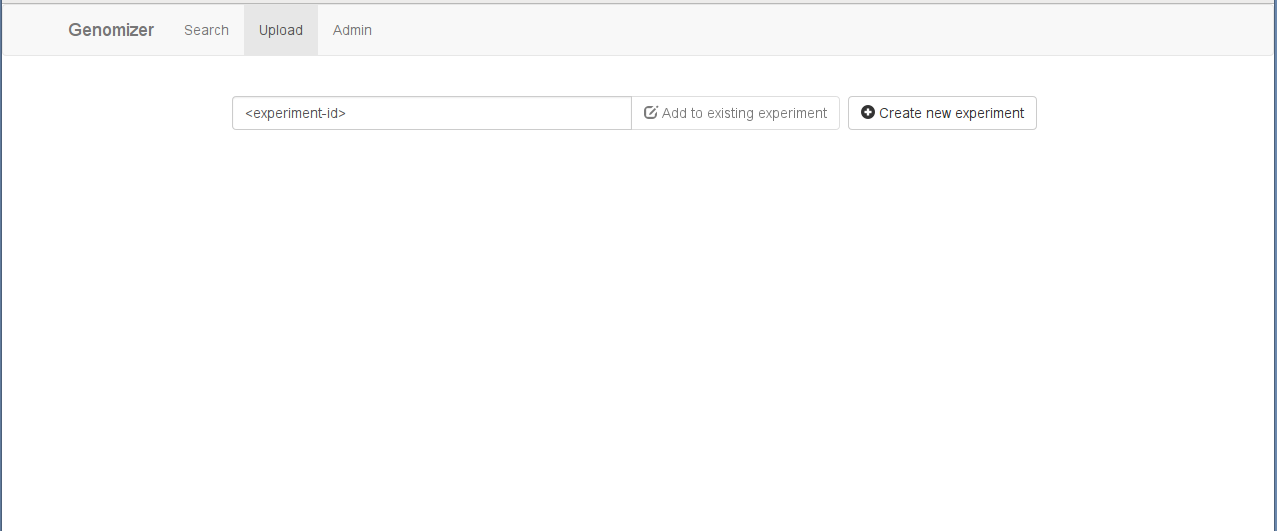
\includegraphics[width=1\textwidth]{web_upload_uploadView.png}
\caption{\label{fig:web_upload_uploadView}The upload view.}
\end{figure}

When the user presses the upload tab in the navigation bar the view in \refer{fig:web_upload_uploadView} will appear. The user has the option to create a new and fresh experiment or to load an existing experiment by entering its experiment ID. 
%figure X8
\begin{figure}[h]
\centering
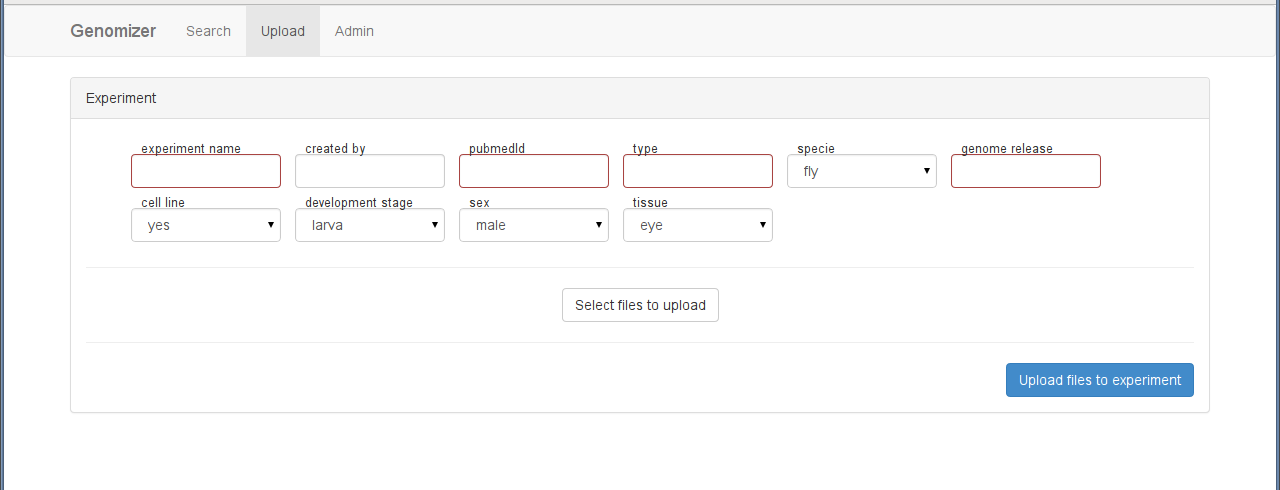
\includegraphics[width=1\textwidth]{web_upload_newExperiment.png}
\caption{\label{fig:web_upload_newExperiment}Creating a new experiment.}
\end{figure}

After clicking the “Create new experiment” button the view in \refer{fig:web_upload_newExperiment} will appear. Here the user can input the annotations for the experiment through either freetext fields or drop-down lists. If a freetext field has a red border around it, that annotation is required and no files can be uploaded before it has been filled in. The user can also browse for local files to upload by clicking the “Select files to upload” button. 
%figure X9
\begin{figure}[h]
\centering
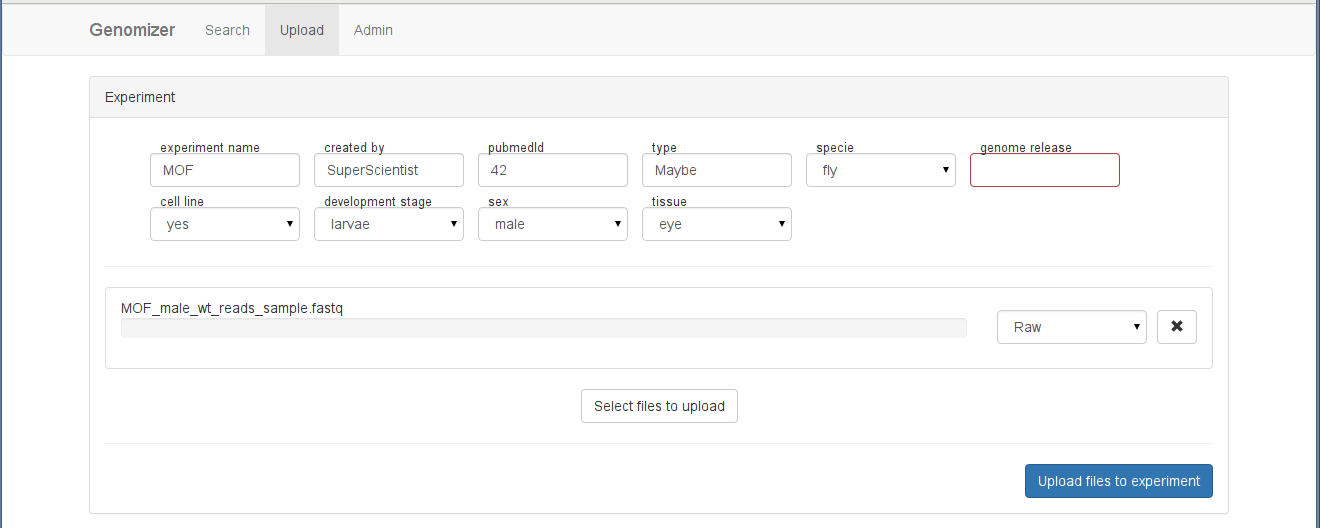
\includegraphics[width=1\textwidth]{web_upload_fileUpload.png}
\caption{\label{fig:web_upload_fileUpload}File selected for upload.}
\end{figure}
 
When the user has selected files, they will appear below the annotations as in Figure \refer{fig:web_upload_fileUpload}. The file’s name is displayed in the top left corner. On the right side there is an option to select what type of file is being uploaded and an option to remove the file from the experiment.

When the user is done selecting files and annotations it can click the “Upload files to experiment” button. The files will then be sent to the server with the specified annotations (this functionality might not be fully working by the time this was written).

\subsubsection{Systemadministration view}

This part of the web application is only accessible if the user have administrator-rights. It is integrated with the rest of the web UI and accessible through an admin-tab. The administrator can through this site see all existing annotations, add new annotations and delete existing ones.
The startpage of this section has a Create new annotations button, a list of existing annotations in the database and an edit button per existing annotation. 
The view currently looks like in figure \refer{adm__web_annotationView}. 

\begin{figure}[h]
 \addImage{web_sysadminAnnotationView.jpg}
 \caption{The startpage for the administrator in the web client}
 \label{adm__web_annotationView}
\end{figure}

For each annotation in the annotations list, an Edit button is available. 
When pressed, it will take you to a page in which you can edit the selected annotation to change its name, 
type and whether it is forced (See \refer{adm_web_editView}). 

\begin{figure}[h]
 \addImage{web_sysadminEditView.jpg}
 \caption{The edit annotation view}
 \label{adm_web_editView}
\end{figure}
\newpage
In the edit page the admin can see the attributes of the chosen annotation and is able to delete the chosen annotation.

If the admin clicks on Create new annotation from the admin startpage, another view will open with the following structure:
\begin{itemize}
 \item Annotation Name
 \subitem Admin can enter a name for the annotation
 
 \item Annotation Types
 \subitem Yes/No/Unknown - this will create a drop-down list with those three options.
 \subitem Freetext - will create an annotation that the users will be able to enter anything.
 \subitem Drop-down list - will enable a fourth field enabling the admin to enter which items that this list will contain.
 
 \item Forced Annotation
 \subitem Admin can choose if the new annotation should be forced for users to enter. 
\end{itemize}

A Create Annotation will, if all necessary information has been entered, result in the annotation to be added to the database. Otherwise the admin will be alerted of the mistake and nothing will be created.
\newpage
A back button which takes the user back to the annotations start page is also available in this view. In figure \refer{adm_web_createView} the create annotation view can be seen.

\begin{figure}[t]
 \addImage{web_sysadminCreateAnnotation.jpg}
 \caption{The view for administrators where new annotations can be created}
 \label{adm_web_createView}
\end{figure}

\subsection{Setting up the application}
To setup the application, move the content of the folder called app in genomizer-web to the desired location from where the application should be run. To run the webpage open a web browser and enter the url to the folder which contains the \texttt{index.html} file(where the content of app was placed).
Ex. given that the genomizer-web folder is placed in my home folder and i want to put the webpage in a folder called public\_html which is also in my home folder. In linux i do the following steps.
\begin{enumerate}
	\item Navigate to the app folder: \texttt{“cd ~/genomizer-web/app/”}
	\item Move the contents of app to the folder called public\_html:\\ \texttt{“mv * ~/public\_html/”}
	\item Given that the url to the pubilc\_html folder is: \\ \filePath{“www8.cs.umu.se/~c11abc/”}
	\item To run the application start a web browser and type \\ \filePath{“www8.cs.umu.se/~c11abc/”}
\end{enumerate}
This will open the webpage in the browser.
